\chapter{Analysis}

\section{Product Opportunity Assessment}

Product opportunity assessment is a helpful procedure to separate the wheat from the chaff. It points out the real pressing issues that are mission critical for the company.

\begin{enumerate}
	\item \emph{What problem are we trying to solve?}
	\item[] Enabling alignment of business language and user interaction reporting is a key part to a success of a new product. No commercially successful platforms allow such alignment, not even any higher semantic analysis. 
	\item[] In a regulatory market it is vital to have an option of storing the user data on custom servers. No such option along with the higher-level analysis is currently available at the market.
	\item[] There is no standardized toolkit and thus the lack of interchangeability between tools tends to end up with a vendor lock-in.
	
	\item \emph{For whom do we solve that problem?}
	\item[] 	For all departments in the company that are participating in product development, top to bottom. From setting a business goal to defining the needs, while also helping the developers and the designers.
	
	\item \emph{How will we measure success?}
	\item[] Having gathered data that is securely placed on custom servers. Data that is united and connected by shared domain vocabulary, ready to be analyzed and visualized in order to draw conclusions.

	\item \emph{What alternatives are out there?}
	\item[] There is some proprietary software on the market, but none is flexible enough for the defined needs.

	\item \emph{Why now?}
	\item[] The competitors \cite{data-driven-pharma} are really getting into the data-driven decisions. The intention is not to gather as much data as possible, but to generate valuable insights as soon as possible in order not to fall behind the competition.

	\item \emph{What factors are critical to success?	}
	\item[] Alignment of all departments participating in software development in a non-invasive fashion. It is critical to primarily focus on helping the departments to connect with each other.
	\item[] The ability to run the whole solution on custom servers and have total control over all gathered data.
	
\end{enumerate}


\section{Regulated environment constraints}

Regulated markets, especially pharmaceuticals have multiple rules that need to be carefully followed in order to be allowed to use new IT products. Not only is important how much value does the final product bring to the end user, but also how data storage is handled and how prone it is to exploitations and attacks. 

From development process point of view it is equally important to follow specific guidelines and processes during the development phase. Each step has to be carefully documented and approved by specific audit department. For that reason, most of the big pharmaceutical companies use the waterfall model - SDLC (= Software Development Life Cycle), which enables companies to follow specific steps in order to get their software product certified. This all hassle is not for the sake of bureaucracy, it is to protect the customers and increases the level of tracability of a problem, should one ever occur. After all, it is their private data that goes on the server, so it is imperative that it is safe.


\section{Existing Tools}

I will now analyze and assess the tools available on the market. I'll focus primarily on the flexibility of the deployment and their analysis features. Anything else has a minor priority.

\subsection{Google Analytics}

Google Analytics is by far the most popular and widely used framework for monitoring user interactions in applications. It reports everything the developer wishes to. By default it does not report anything - the tool has to be activated during application start. Then each action needs to be hard-coded in the code. An action can be two things - the first one is after a certain user activity has happened - a press of a button, pulling down a list to refresh the data etc. One thing gets reported - "this event has happened". The second one is more open - an identifier is set to an item, let's say, a button. Whatever happens with that button gets reported, be it touch, swipe or anything else.

\begin{figure}[!ht]
	\centering
	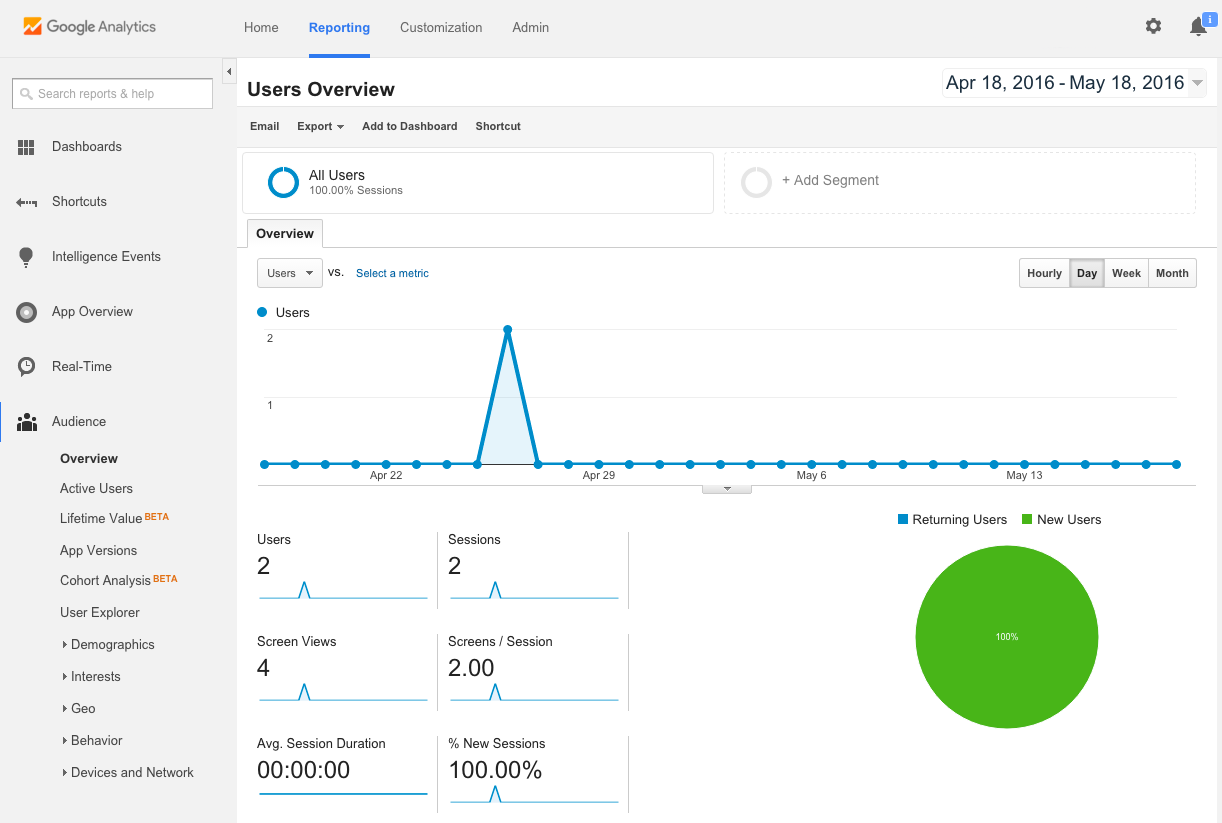
\includegraphics[width=0.65\textwidth]{figures/analytics}
    \caption{Google Analytics Dashboard}
\end{figure}

The dashboard website is very detailed and responsive. All data is nicely visualized in graphs and corresponds well with the whole GA ecosystem. Higher order semantics is remotely possible via definition of complex queries and dashboard setups. User management is very rich and enables forming multiple roles for different users. The main problem is, unfortunately, that all data goes to Google. There is no option of having the engine run on custom servers. All code is closed source and that simply wouldn't go through any risk assessments because Google might be sending the data to anywhere in the world.

Data is accessible via REST API, but registration for it is required (it is not possible for a "normal" user to start using the REST API). Single user account is free, enterprise account is paid.

\subsection{Google Tag Manager}

Google Tag Manager is a tag management system that allows quick and easy update of tags and code snippets in a mobile application. It allows adding and updating AdWords, Google Analytics, etc. from the Tag Manager user interface instead of editing the code.

A tag is a snippet of code that sends information to Google. It is not necessary to wire it up in code - it works through configuration files from the admin user interface.

Tag Manager is deployed in conjunction with the Firebase SDK, with support for both Android and iOS. The container replaces all other manually-coded tags in the mobile application, including tags from AdWords, Google Analytics etc. It basically builds on top of Google Analytics to make the integration a little easier. It is aimed to be used by people focused mainly on marketing, thus the tool itself serves as an overall performance dashboard. It allows them to create complex tags in a short period of time. Unfortunately it works well only on the web - the tags have to be hard-coded in mobile applications.

\newpage

\begin{figure}[!ht]
	\centering
	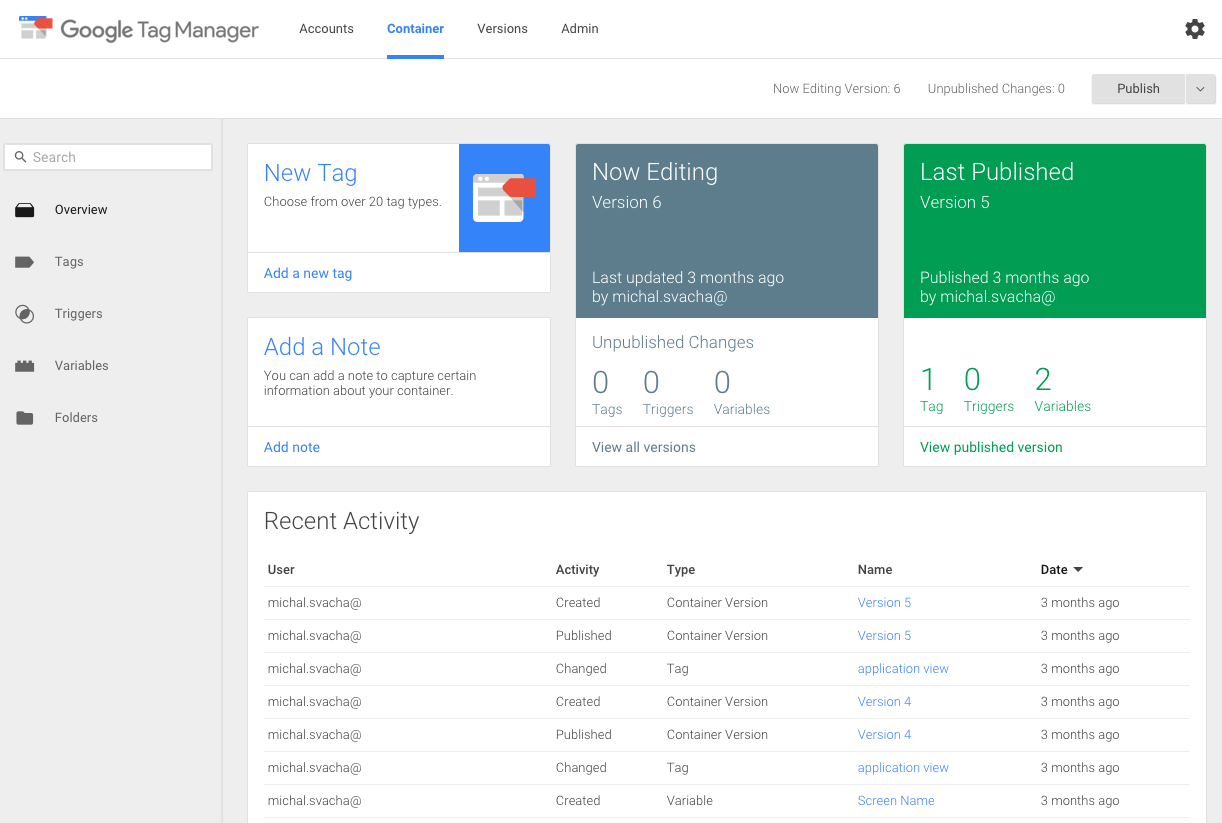
\includegraphics[width=0.65\textwidth]{figures/tagmanager}
    \caption{Google Tag Manager Dashboard}
\end{figure}

The dashboard is similar in style to the Google Analytics one. Tags can be created, modified and linked with a specific Google Analytics query. The same as for Google Analytics holds for Google Tag Manager - everything is closed source and runs exclusively on Google's servers.

\subsection{Teallium}

TBD

\subsection{Fabric (formerly Crashlytics)}

Crashlytics was also a star framework. Acquired by Twitter, it is now a vital part all purpose platform - Fabric. Fabric is aside from a reporting tool a full featured developer platform used for variety of tasks and obstacles a developer may face - even beta version distribution that has always been a problem for iOS developers. The Crashlytics reporting has been taken a step further and is not only about reporting crashes. It also reports overall statistics, like Google. One nice feature Fabric has is by acquiring AppSee - a way of visualizing user movement in the app through the usage data. A video of steps users take in their app gives the developer a new perspective on how the app is used.

The source code is closed source and all of the statistics run ot Twitter servers. Data is NOT accessible. The whole platform is free to use. Registration is required along with installation of a custom program to install the framework parts in existing projects.


\subsection{App Pulse (formerly Pronq)}

App Pulse is a "new feature by acquisition" - acquired by HP in 2014, it is now part of the portfolio of the new Hewlett Packard Enterprise. It lets users try out their 30-day trial and then charges for everything (no free version).

App Pulse is very different from GA in a way that it reports everything at all times. The usage is fairly low - tens of kilobytes per week, but it is very thorough. Screen time, actions, movements - it is all there. No setup is required for the start. The SDK they supply simply has to be dragged and dropped in Xcode project and then it starts working out-of-the-box. The only issue is the need to have consistent naming of all views, labels, buttons etc. - as it does everything on its own, without hooking up the actionable items to the framework manually, it can be hard to determine which button was which.

The tools are closed source and all of the statistics run on HP servers. No API is provided.


\subsection{Crittercism}

Crittercism doesn't stand out from previously mentioned tools - has their own servers, SDK and works seemlessly. Has some more benchmarking than others, and seems very enterprise oriented - they enable 3rd party API integration into their system to see performance of other APIs used in the application to really find what can be the bottleneck of the app's performance.

The tools are closed source and all of the statistics run on their servers. API is provided.


\subsection{New Relic}

New Relic somewhat differs in a sense that as the only platform there is a mention on their website about "specific needs" - maybe custom server can be provided. Otherwise it is the same strategy - SDK installed in every app and statistics gets reported periodically. Nice alerting system is optionally provided - when crash occurs, web hook to ticketing system can be defined to streamline bug reports.

The SDKs are open source, the analytics runs on their servers (~ possibly 'not only'). No API is provided.


\subsection{Apple}

The last isn't considered framework, but it should be noticed. As companies fight for data from mobile applications - such as Twitter, who gives out their platform free for everybody, naturally the platform owners strive for keeping all that precious data for themselves. Apple announced at WWDC 2015 new iTunes Connect portal redesign and along with it also a new feature - App Analytics. It is fairly thorough in means of usage, downloads, screen time etc, but overall reporting is still very high level and really far from the code. It seems like it is not meant to be a developer tool at all, because there is no in depth code reporting. There are crashes reported, but not very detailed compared to Fabric.

These statistics are provided to every single developer of iOS apps for free on the iTunes Connect website. There is no framework and naturally Apple keeps all of the data for themselves.


\subsection*{Conclusion on tools}

Why are they bad etc etc.